\chapter{DreamDateのプロトタイピングと機能}
\label{chap:search}

この章ではDreamDateのシステムの概要、利用方法 について述べる。

\section{機能}
 現在、仮想現実を体験すべくヘットマウントディスプレーなどの様々なツールが開発されている。そこで睡眠中の夢を自由自在にコントロールする方法があれば誰もがより簡単に仮想現実を体験できるのではないかと考えた。\\
 睡眠中にユーザがの思い出と関連した音を流すことで、その音に基づいて夢を見ることを促進するスマートフォンアプリDreamDateを試作した。ターゲットと考えているユーザは日々のストレスから解放されたい人、懐かしい思い出をもう一度体験したい人、物理的に会えない人と会いたい人などである。\\
 DreamDateには3つ主要な機能がある。一つ目は寝る前に印象に残っている記憶に関する写真と映像を表示する機能。二つ目は睡眠中にレム睡眠を検出し、記憶を連想させる音を流す機能。例えば特別な誰かを連想する音、旅行中によく聞いていた曲、最寄り駅の音楽、好きな映画のサウンドトラックなどがある。三つ目は起床後に夢について記録する夢日記機能である。ユーザには睡眠前にスマートフォンを画像\ref{DreamDateImage}のように枕の横に置いてもらう。\\
アプリを使用して実験をした結果、DreamDateには欠点があることがわかった。それはユーザが自分の記憶を連想する音を探し出して登録しなければならないということ。例えば海の音を聞けば海の夢を見れるということではない。しかし実際に海に行った特別な記憶がある人であれば、海の音を流せばその夢を見る確率は比較的に上がる。\\
DreamDateは開発途中でまだAppストアには掲示していないが、githubからソースコードを入手することができる。iOSスマートフォンを持っていて、Apple Developerの登録をしている人であればインストールできるようになっている。

\begin{figure}[htbp]
\begin{center}
\includegraphics[width=14cm]{eps/dreamDate02.eps}
\caption{DreamDateの配置}
\label{DreamDateImage}
\end{center}
\end{figure}

Xcode 上で openframeworks ライブラリを利用して、iPhoneの加速度センサーを利用した体動検知アプリケーションを制作した。睡眠時に枕の横に iPhone を置いて、体動(寝返り)による寝具の動きを検知して加速度を測定す る。\\
 まずベッドの硬さは人により違うため、キャリブレーションをしてもらう。アプリ起動後ユーザにはiPhoneを横に置いた状態で15秒間静止してもらう。x軸の加速度を毎秒記録、1秒前の加速度との差分を導き出す。20秒間、x軸の差分の中での最大値を閾値として設定する。y軸とz軸の測定をしなかったのはx軸だけでも十分寝返りを特定できるためである。ベッドで寝てから睡眠に至るまで平均的に10分から20分かかるとされているため、スタートボタンが押されてから20分後に加速度センサーによる体動のモニタリングが開始される。こうすることで、寝ようとしている最中に音楽がならないようにする。モニタリングが開始されてからはノイズを除去するために、毎20秒の平均値が出される。その平均値が閾値に比べて高くなった時に寝返りをしたと判定する。寝返りを打つ時は睡眠段階がレム睡眠からノンレム睡眠に、あるいはノンレム睡眠からレム睡眠への切り替わったときだ\cite{negaeri}。そのためレム睡眠の間はあらかじめ設定していた音楽が図\ref{melodyGraph}で示したオレンジのタイミングで流れる。レム睡眠時にのみ音楽を流したのは常に音楽が流れていると睡眠が害され睡眠サイクルが崩れて体調不良などを引き起こす可能性が高くなるためである。

\begin{figure}[htbp]
\begin{center}
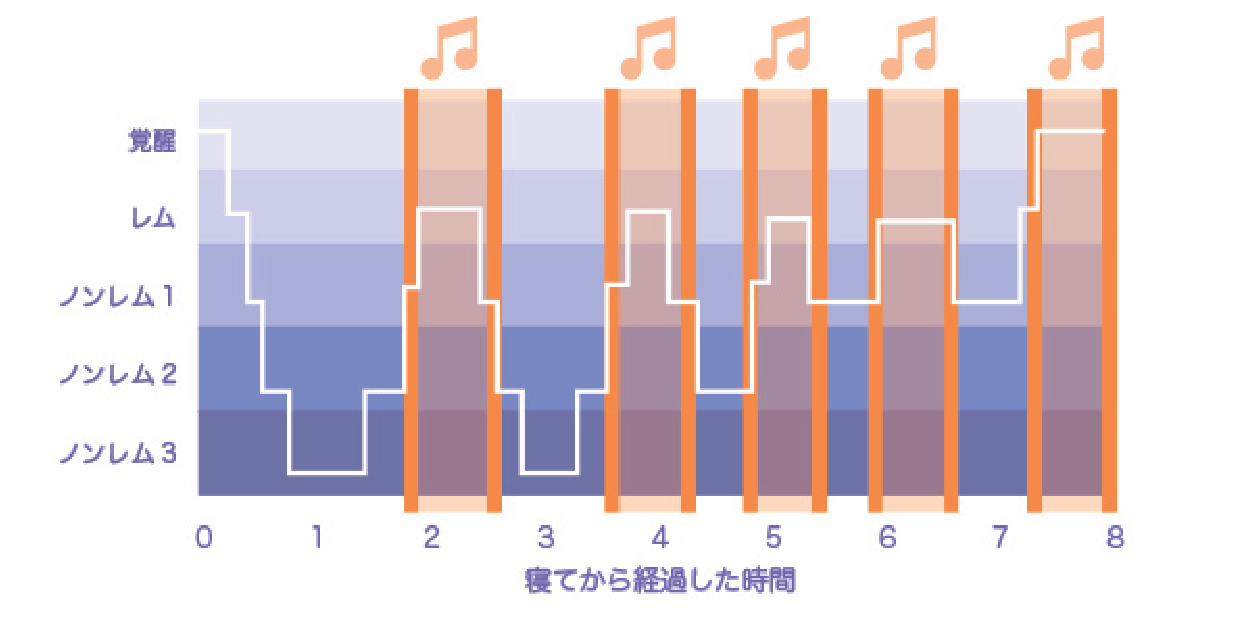
\includegraphics[width=15cm]{eps/remNonrem.eps}
\caption{音刺激提示のタイミング}
\label{melodyGraph}
\end{center}
\end{figure}

一晩中のx軸の数値、音楽の再生状況、夢日記の結果はデータベースをクラウドであるParseに保存する。図\ref{system}に一連のプログラムの流れを記載する。
\begin{figure}[htbp]
\begin{center}
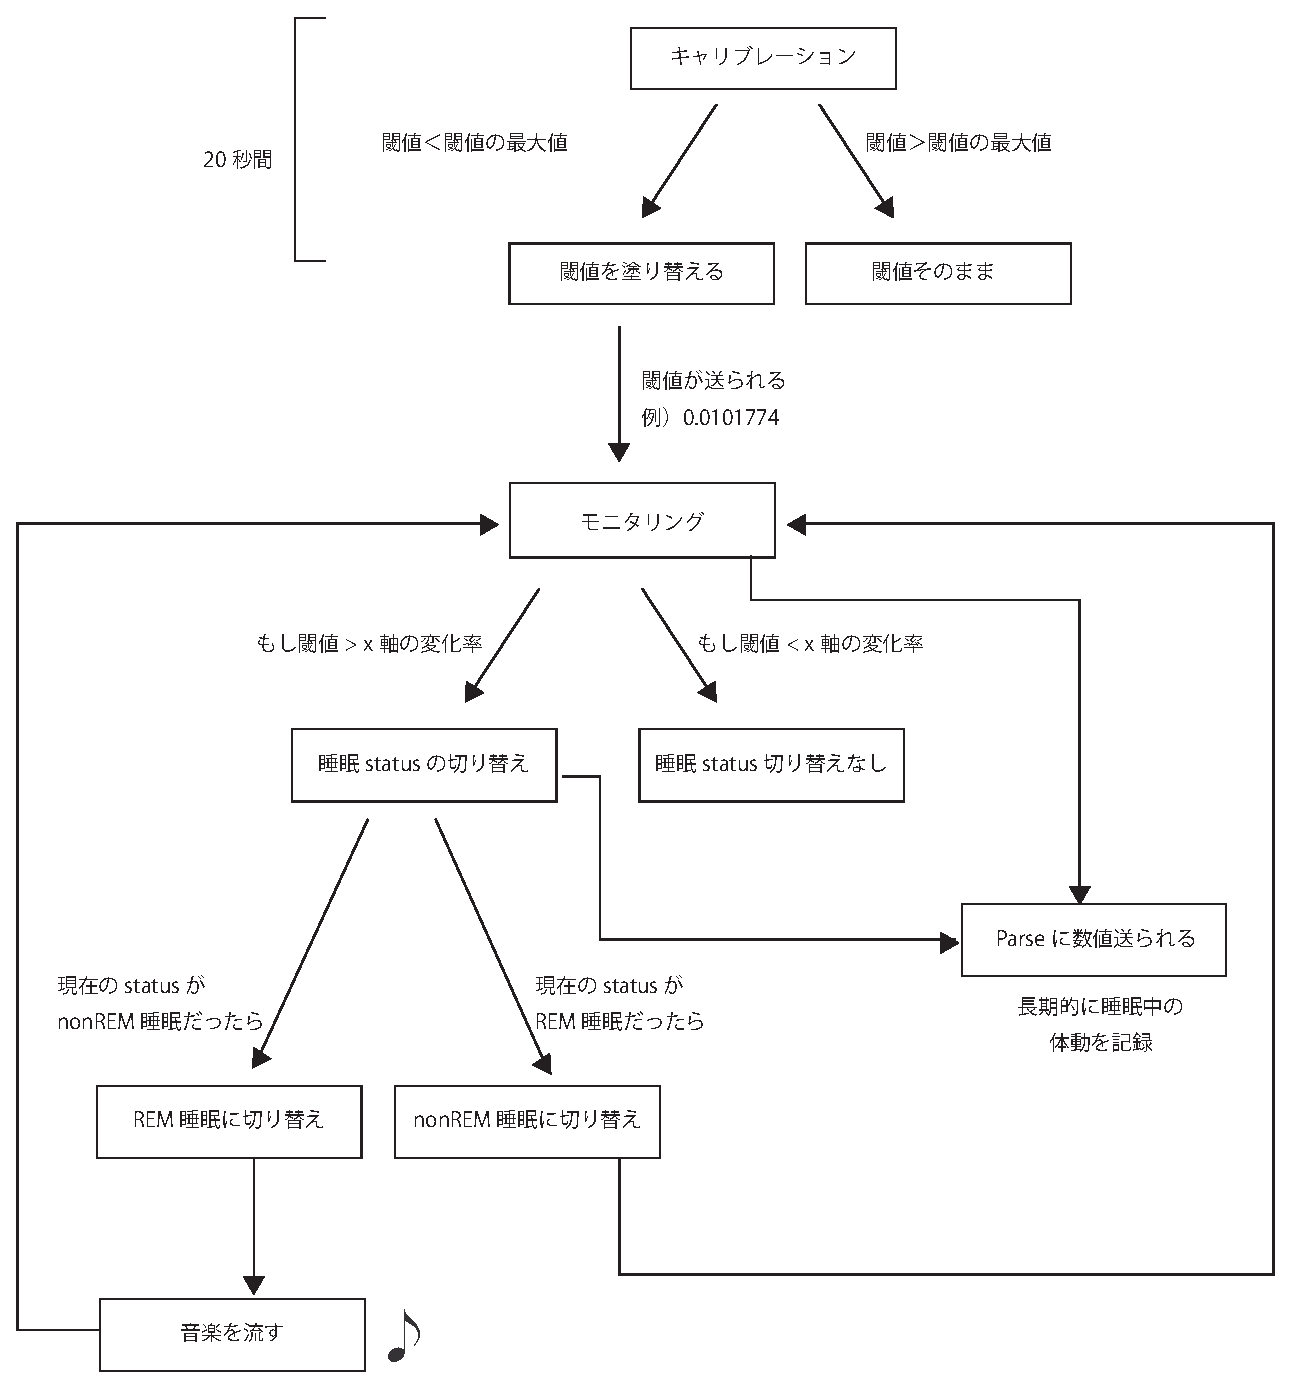
\includegraphics[width=15cm]{eps/system.eps}
\caption{DreamDateのフローチャート}
\label{system}
\end{center}
\end{figure}

\section{利用方法}
 ユーザには予め記憶を思い起こさせる音と画像を登録してもらう。音選びは適している音声と適さない音声があるため注意する必要がある。使用してはならない音は人の声である。特に喋りかけてくるような内容の音声は、ユーザを起こしてしまう可能性が高いということが実験結果から分かった。詳しくは第6章で述べる。逆に適している音は繰り返しある環境下で聞いていた音である。
 アプリの起動後、\ref{le01}のような画面が表示される。そこには「自動ロック機能をOFFにする」「音量は1〜3に設定する」やiPhoneの置く位置などの指示が書かれている。次に\ref{le02}の画面に遷移し、ユーザの思い出に関連性のある画像を表示する。ここでは寝る前に記憶の情景を思い出す機会を与えている。そして\ref{le03}の画面では思い出の音楽が流れる。音楽を聴きながら、旅先での空間、香り、音の細部までを思い出して、気持ちを落ちつかせて瞑想状態に入ってもらう。次に\ref{le04}の画面に移動しユーザは実験日を選択する。実験日1は曲が流れない夜。実験日2はレム睡眠中ずっと曲が流れる。実験3は起きる前のレム睡眠のときのみ音が流れる。次に\ref{le05}寝る前にアプリを起動してスタートボタンを押し、起動させたままスクリーンを伏せて枕の横に置く。20〜30分間後にDreamDateの加速度が起動をし一晩中ユーザの体動のトレッキングが行われ、レム睡眠を検知すると音楽がなる。起床後\ref{le06}の画面で、ユーザは起床すると夢の内容を忘れないように日記に投稿する。

\begin{figure}[htbp]
 \begin{minipage}{0.45\hsize}
  \begin{center}
   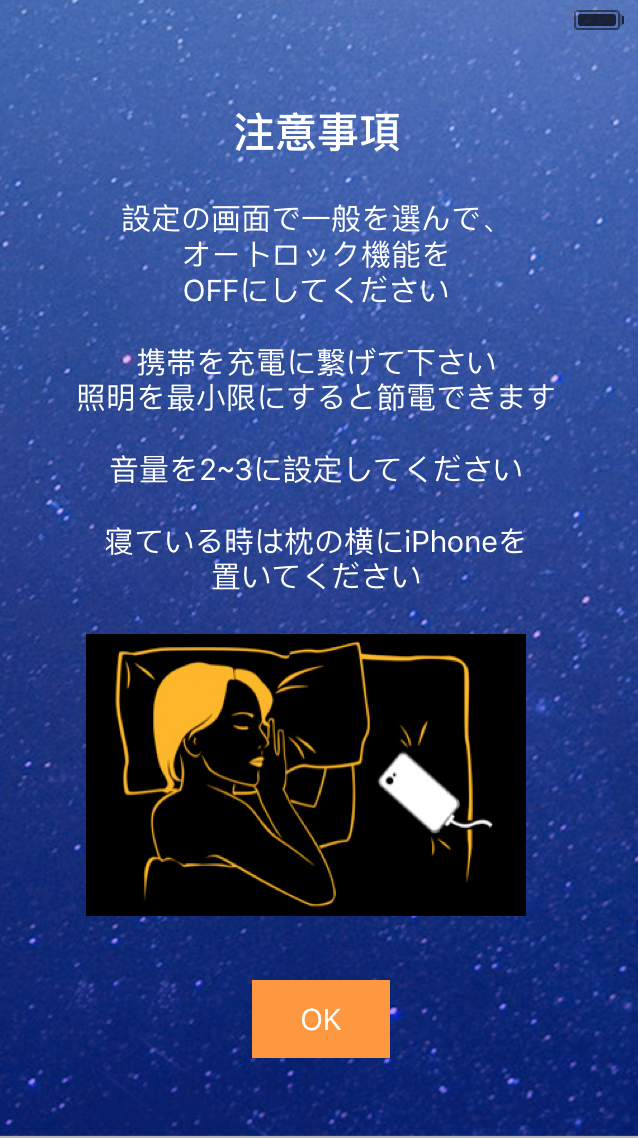
\includegraphics[height=90mm]{eps/AppIntro.eps}
  \end{center}
  \caption{起動画面}
  \label{le01}
 \end{minipage}
  \begin{minipage}{0.45\hsize}
  \begin{center}
   \includegraphics[height=90mm]{eps/AppMemoryImages.eps}
  \end{center}
  \caption{思い出の画像を表示}
  \label{le02}
 \end{minipage}
\end{figure}
\begin{figure}[htbp]
 \begin{minipage}{0.45\hsize}
  \begin{center}
   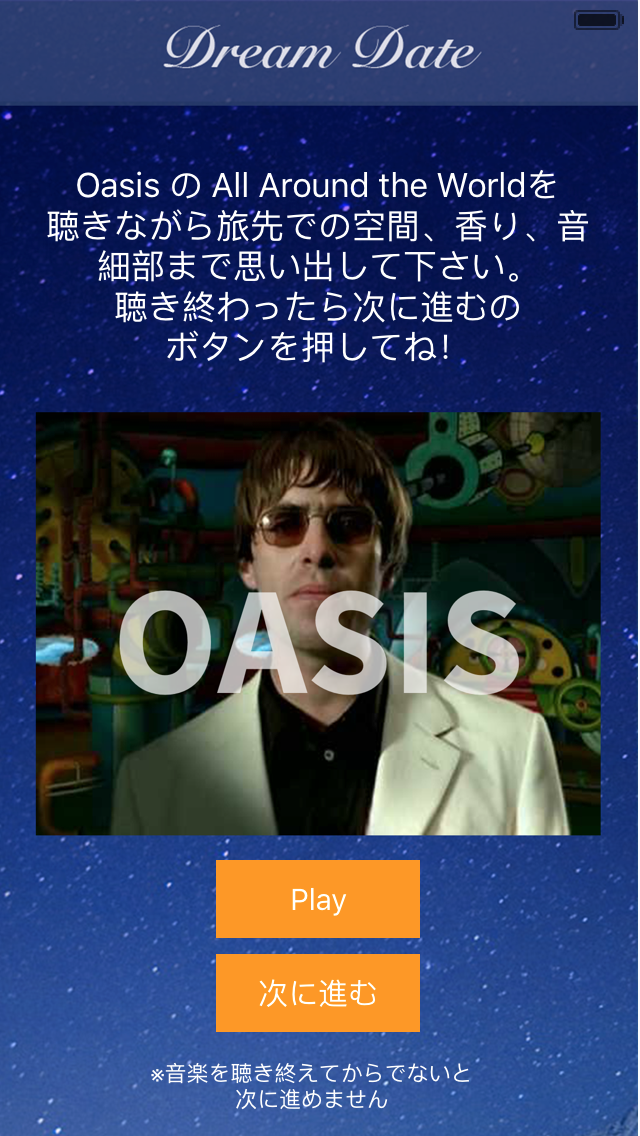
\includegraphics[height=90mm]{eps/AppMusicPlay.eps}
  \end{center}
  \caption{思い出に関連した音刺激の提示}
  \label{le03}
 \end{minipage}
 \begin{minipage}{0.45\hsize}
  \begin{center}
   \includegraphics[height=90mm]{eps/AppExperienmentType.eps}
  \end{center}
  \caption{実験日選択ボタン}
  \label{le04}
 \end{minipage}
\end{figure}

\begin{figure}[htbp]
 \begin{minipage}{0.45\hsize}
  \begin{center}
   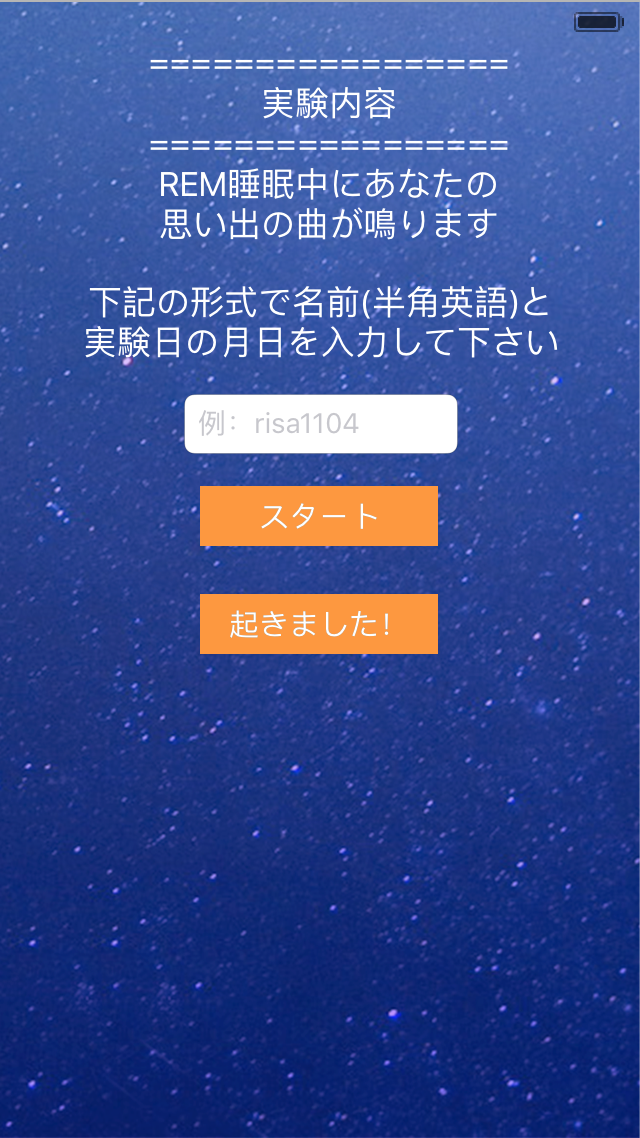
\includegraphics[height=90mm]{eps/AppStart.eps}
  \end{center}
  \caption{睡眠開始ボタン}
  \label{le05}
 \end{minipage}
 \begin{minipage}{0.45\hsize}
  \begin{center}
   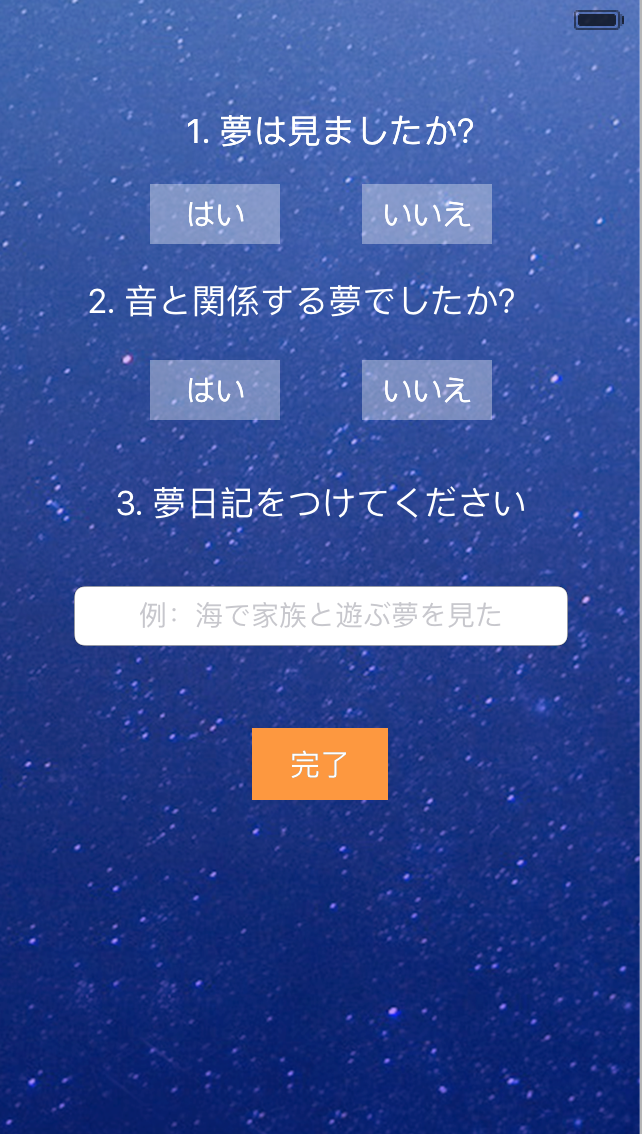
\includegraphics[height=90mm]{eps/AppDiary.eps}
  \end{center}
  \caption{夢日記記入ページ}
  \label{le06}
 \end{minipage}
\end{figure}